\documentclass[tikz,border=0pt]{standalone}
\usepackage[american]{circuitikz}
\usetikzlibrary{arrows.meta,calc,positioning,decorations.pathmorphing,patterns}
\definecolor{zyloTeal}{HTML}{174A5B}
\definecolor{zyloTealTwo}{HTML}{246B7A}
\definecolor{zyloInk}{HTML}{1F2933}
\definecolor{zyloSoft}{HTML}{EAF4F4}
\definecolor{zyloPaper}{HTML}{F8FAFB}
\definecolor{zyloLine}{HTML}{44606B}
\definecolor{zyloOrange}{HTML}{D97706}
\begin{document}
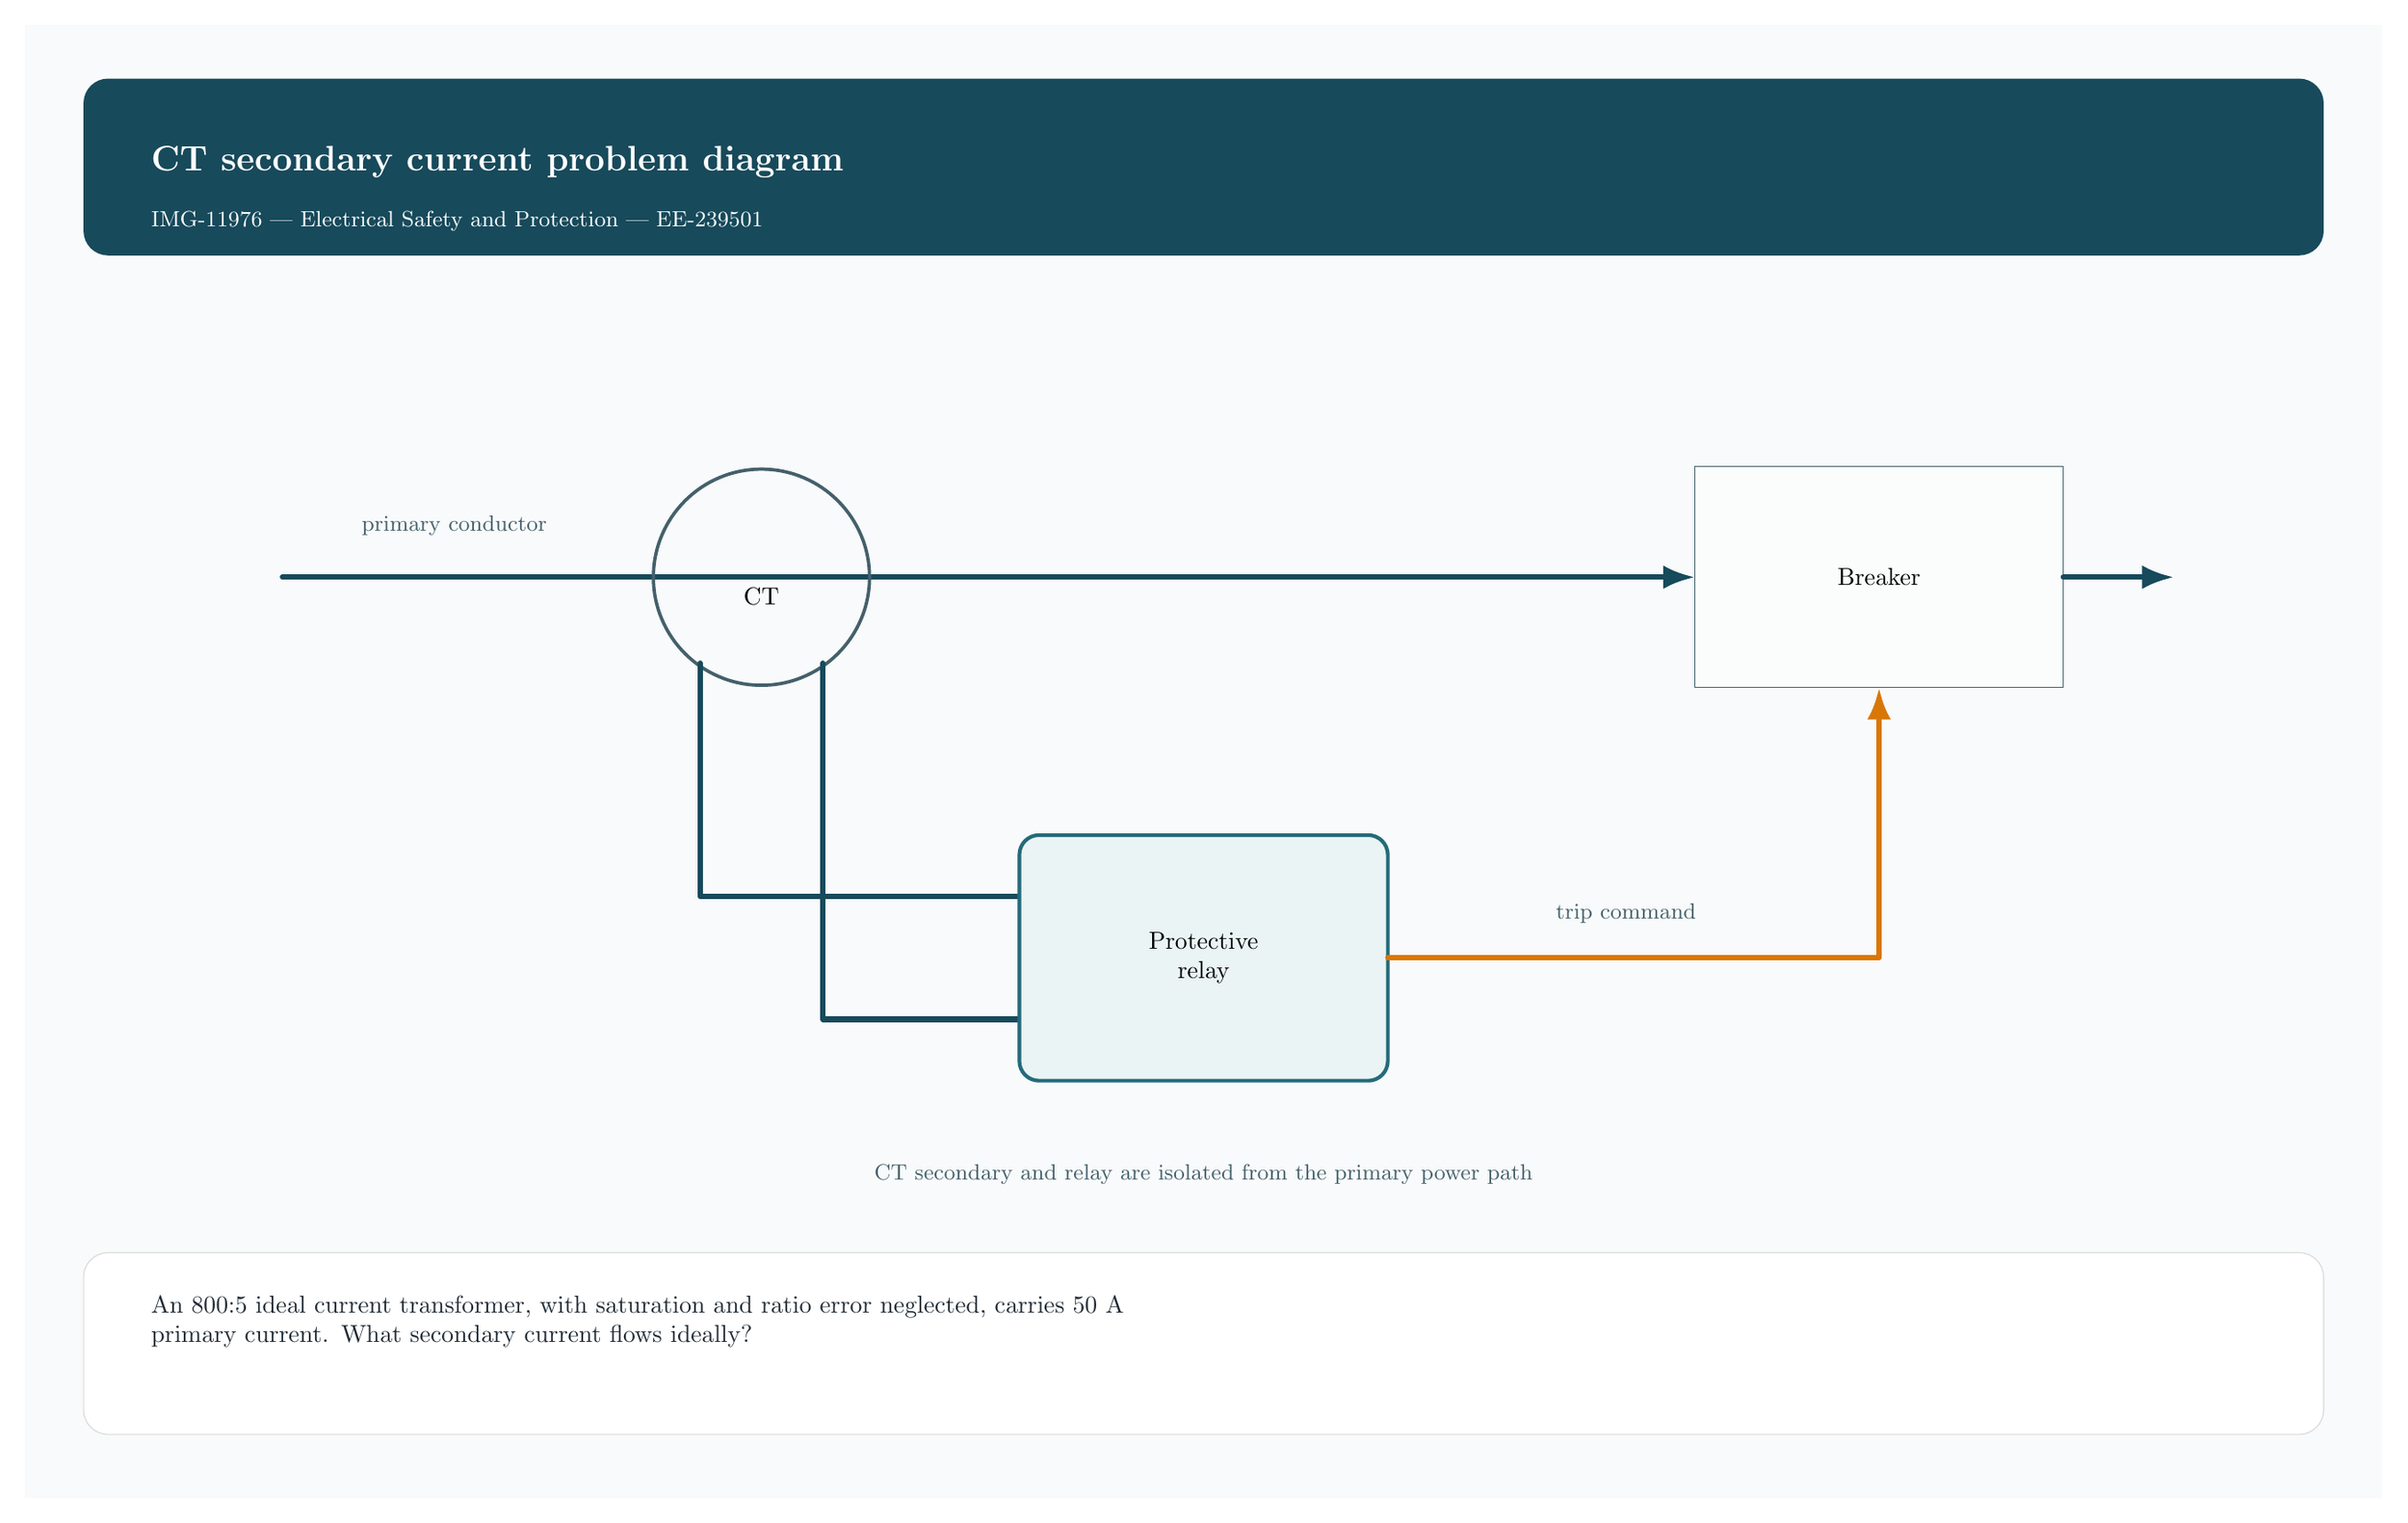
\begin{tikzpicture}[x=1pt,y=-1pt,>=Latex,line cap=round,line join=round]
\path[fill=zyloPaper] (0,0) rectangle (960,600);
\path[fill=zyloTeal,rounded corners=10pt] (24,22) rectangle (936,94);
\node[anchor=west,text=white,font=\bfseries\Large] at (48,56) {CT secondary current problem diagram};
\node[anchor=west,text=white!82,font=\small] at (48,80) {IMG-11976 | Electrical Safety and Protection | EE-239501};
\tikzset{wire/.style={draw=zyloTeal,line width=2.2pt},thinwire/.style={draw=zyloLine,line width=1.35pt},accent/.style={draw=zyloOrange,line width=2.2pt},box/.style={draw=zyloTealTwo,fill=zyloSoft,line width=1.5pt,rounded corners=8pt}}
\draw[wire,->] (105,225) -- (680,225); \node[font=\small,text=zyloLine] at (175,204) {primary conductor};
\draw[thinwire] (300,225) circle (44); \node at (300,233) {CT};
\node[draw=zyloLine,fill=white!80!zyloSoft,minimum width=150pt,minimum height=90pt] at (755,225) {Breaker}; \draw[wire,->] (830,225) -- (875,225);
\draw[wire] (275,260) -- (275,355) -- (405,355); \draw[wire] (325,260) -- (325,405) -- (405,405);
\node[box,minimum width=150pt,minimum height=100pt,align=center] at (480,380) {Protective\\relay};
\draw[accent,->] (555,380) -- (755,380) -- (755,270); \node[font=\small,text=zyloLine] at (652,362) {trip command};
\node[font=\small,text=zyloLine] at (480,468) {CT secondary and relay are isolated from the primary power path};
\path[draw=black!15,fill=white,rounded corners=10pt] (24,500) rectangle (936,574);
\node[anchor=west,text width=860pt,align=left,text=zyloInk,font=\normalsize] at (48,528) {An 800:5 ideal current transformer, with saturation and ratio error neglected, carries 50 A\\primary current. What secondary current flows ideally?};
\end{tikzpicture}
\end{document}
